% ===================================================================================================================
% Section: Experiments (25%). Needs: amsmath, booktabs, graphicx, natbib; \graphicspath{{figures/}}; references.bib.
% Every figure and table sits in this section, next to the text that cites it.
% Sources: epills/outputs/runs/*/eval/*.json, docs/stage2_results.md, docs/evidence.md.
% ===================================================================================================================
\section{Experiments}
\label{sec:experiments}

\subsection{Data and evaluation setup}
\label{sec:setup}

\paragraph{Training source and identity units.}
The primary source is the National Library of Medicine (NLM) Computational Photography Project for Pill Identification (C3PI) collection~\citep{yaniv2016nlm}. Its consumer-image list contains 40,882 entries, including 295 exact repeats, leaving 40,587 distinct photographs that were successfully cropped and assigned to partitions. Pill types are defined by nine-digit National Drug Code (NDC9) and product part, giving 2,400 types after package variants are consolidated. Types sharing recorded imprint, shape, colour and size form an \emph{appearance group}, while those without imprint text remain separate. The resulting 2,338 groups define training labels and partition membership, with product identities retained for catalogue retrieval.

Consumer photographs vary in illumination, orientation, visible side and background, with a median of 15 images per medicine and a range of 3--101 in the inventory's NDC9 summary. Studio references provide more consistent views for catalogue matching and augment training groups in runs 3 and 4. Appendix~\ref{app:data} details the count reconciliation, package variants and grouping process, together with the distribution plot in Figure~\ref{fig:data-statistics}.

\begin{table}[!htbp]
\centering\small
\caption{C3PI partitions after removal of repeated entries and successful cropping of all 40,587 distinct consumer photographs. Studio references add 6,198 training crops in runs 3 and 4.}
\label{tab:data}
\begin{tabular}{@{}lrrl@{}}
\toprule
Partition & Groups & Crops & Role \\
\midrule
Training & 1,710 & 29,471 & Representation learning \\
Validation enrolled & 214 & 3,556 & Selection and enrolment \\
Validation unknown & 214 & 3,555 & Rejection calibration \\
Held-out test & 200 & 4,005 & Evaluation on unseen groups \\
\bottomrule
\end{tabular}
\end{table}

\paragraph{Partitioning and preprocessing.}
Groups containing an ePillID fold-4 holdout identity are reserved through NDC9 matching. Remaining groups are randomly divided approximately 80:10:10 between training and the two validation partitions (Table~\ref{tab:data}). Code for split generation checks shared identifiers, exact duplicates and near-duplicate crops. Only references for training groups are added in runs 3 and 4. Each detected pill is framed in a square window of 1.55 times the long side of its bounding box and resized to $224\times224$ pixels. VGG16 inputs use ImageNet channel statistics, while ViT inputs are scaled to $[-1,1]$, with constants given in Appendix~\ref{app:configuration}. Training augmentation is specified in Section~\ref{sec:training}. Figure~\ref{fig:examples} provides representative views.



\begin{figure}[!htbp]
\centering
\begin{minipage}[t]{0.48\linewidth}
\vspace{0pt}\centering
\textbf{(a) C3PI image variation}\\[3pt]
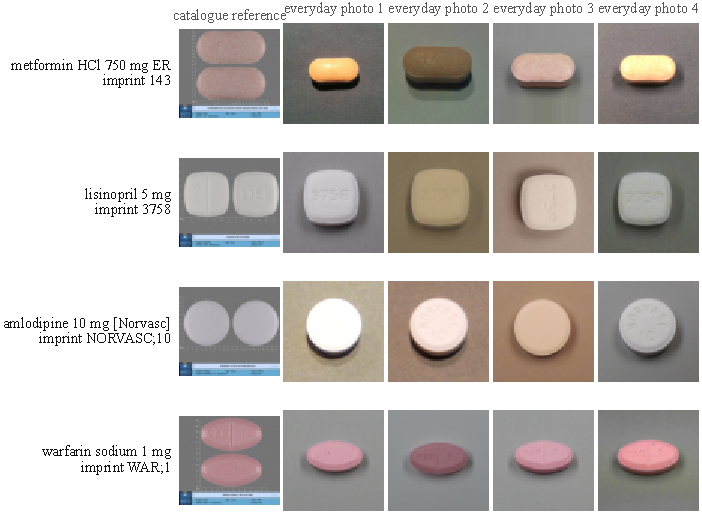
\includegraphics[width=\linewidth]{fig04_qualitative_examples.pdf}
\end{minipage}\hfill
\begin{minipage}[t]{0.49\linewidth}
\vspace{0pt}\centering
\textbf{(b) ePillID side coverage}\\[3pt]
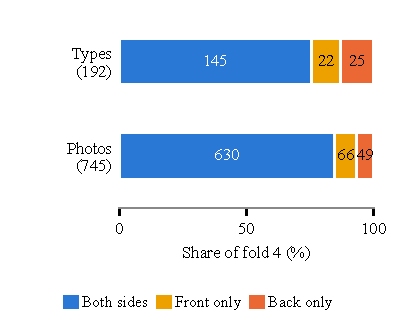
\includegraphics[width=\linewidth]{figD4_epillid_sides_compact.pdf}
\end{minipage}
\caption{Data characteristics. (a) Catalogue references and four consumer photographs for each of four medicines illustrate variation in orientation, visible side and illumination. (b) ePillID fold-4 coverage by side availability, shown for pill types and photographs.}
\label{fig:examples}
\end{figure}

\paragraph{Evaluation sources and catalogue.}
The C3PI holdout comprises 200 appearance groups, whereas the local ePillID release contains 13,532 images of 4,902 types, including 9,804 references and 3,728 consumer images. Fold 4 contains 745 consumer photographs of 192 identities~\citep{usuyama2020epillid}. The official ePillID protocol permits reference images for test types during training, distinguishing it from the strict C3PI evaluation. MEDISEG~\citep{mediseg2026} contributes 8,261 images with 14,069 annotated pills from 32 Hong Kong products. For evaluation with all products enrolled, three single-pill photographs per product form the gallery, leaving 13,973 query pills after 96 enrolment instances are excluded. The median pill long side is 81 pixels, with fifth and 95th percentiles of 27 and 194 pixels in $640\times640$ images. A separate deployment subset has 40 query pills. Product population, scale, cameras and clutter change together, so the external gap cannot be attributed to camera hardware alone. Catalogue identification uses 4,936 US products assembled from C3PI reference images and imprint, shape and colour metadata.

\paragraph{Data use.}
The study uses public image datasets without patient records. C3PI images are restricted to research and development, including when accessed through ePillID, whose MIT code licence does not supersede the image conditions. MEDISEG is distributed under CC BY 4.0, and download instructions for all sources are provided in \texttt{epills/docs/datasets.md}.


\paragraph{Metrics for medication verification.} We simulate patients with 10 enrolled medicines (3 photos each). For the
patient's own pills we report the share \emph{named correctly}, \emph{named wrongly} (an accepted misidentification),
\emph{retake} and \emph{called unknown}; for pills that are not theirs, the share \emph{rejected}. An accepted name can inform subsequent action, whereas unknown and retake outcomes add a further checking step to the workflow. We also report top-$k$ accuracy, area under the receiver operating characteristic curve (AUROC),
ePillID's mean average precision (MAP) and global average precision (GAP), and the reliability of the stated confidence. Intervals are obtained from 1,000 bootstrap replicates, resampling medicine groups with replacement and
retaining all their repeated query appearances. The 2.5th and 97.5th percentiles define the reported 95\% intervals.

\paragraph{Gallery simulation.} The evaluation code samples 1,000 galleries using seed 0. Within each
gallery, ten eligible medicines are sampled without replacement and three enrolment images are selected per
medicine. All remaining images of those medicines are used as enrolled queries. Enrolment images are excluded
from queries within that gallery. Up to 200 images of medicines outside the gallery are sampled without
replacement as foreign queries. Identities and photographs can recur across galleries. Percentages are computed
by pooling query rows rather than averaging gallery percentages. For MEDISEG, enrolment is restricted to
single-pill images. The simulation and bootstrap procedures are implemented in
\texttt{epills/src/epills/training/eval/openset.py}; they were inspected for this report.

\paragraph{Baselines.} (i) Run 1: the same network with a common recipe (new layers at $10^{-3}$, no margin
warm-up). (ii) The published ePillID models~\citep{usuyama2020epillid}. (iii) Look only versus look plus imprint, for
the gallery and the catalogue.

\subsection{Main results}
\label{sec:main}

Table~\ref{tab:main} reports results under the strict protocol. In the conditions
it was trained for, the served model (run 4) names 76.0\% of a patient's own pills correctly and only 0.04\% wrongly
(95\% confidence interval 0.02--0.07\%), while rejecting 94.8\% of pills that are not the patient's (Figure~\ref{fig:openset}a). The
imprint check raises correct names to 78.3\% (wrong 0.06\%) by settling retakes. These rates of wrong naming use enrolled queries as their denominator. With the imprint
pipeline, 3.5\% of foreign queries receive an accepted gallery identity and 94.8\% are called unknown;
the remainder request a retake (approximately 1.7\%, inferred from rounded reported rates). Thus the
0.06\% error among enrolled queries is not the overall rate of accepting a wrong medicine. Catalogue identification improves from 71.6\% to 80.2\% top-1 and from 91.7\% to 94.4\% top-5 with imprint re-ranking. Adding training-group references in run 3 raises strict ePillID MAP@1 from 13.7\% to 37.1\%. Run 4's acquisition augmentation gains 6.4 percentage points on MEDISEG while reducing C3PI top-1 by 1.2 points. Run 4 is the served model.

\begin{table}[!htbp]
  \caption{Test results on medicines never seen in training (\%; 10-medicine galleries, 3 enrolment photos,
    calibrated $\tau$ and $m$). Bottom block: the served pipeline with imprint reading (GPU reader, CPU reader in
    brackets).}
  \label{tab:main}
  \centering
  \small
  \begin{tabular}{@{}lccc@{}}
    \toprule
    & Run 2 & Run 3 & Run 4 (served) \\
    \midrule
    C3PI held-out: top-1 among 200 medicines & 82.0 & \textbf{84.4} & 83.2 \\
    \quad gallery: named correctly / wrongly & 78.6 / 0.1 & \textbf{80.4} / 0.0 & 76.0 / 0.04 \\
    \quad other medicines rejected & 94.2 & 94.1 & \textbf{94.8} \\
    MEDISEG: top-1 among 32 products & 38.9 & 41.8 & \textbf{48.2} \\
    \quad gallery: named correctly / wrongly & 17.6 / 1.1 & 18.7 / 1.0 & 18.7 / \textbf{0.7} \\
    \quad own called unknown / other rejected & 51.5 / 78.7 & 64.2 / 89.3 & 70.4 / \textbf{93.1} \\
    ePillID strict (no test type in training): MAP@1 & 13.7 & 37.1 & \textbf{42.3} \\
    \midrule
    C3PI gallery + imprint check: named correctly / wrongly & & & 78.3 (77.3) / 0.06 \\
    \quad retake / called unknown & & & 7.2 / 14.5 \\
    \quad foreign: unknown / accepted match & & & 94.8 / 3.5 \\
    Catalogue (4,936 products) + imprint: top-1 / top-5 & & & 80.2 (79.2) / 94.4 \\
    \quad look only: top-1 / top-5 & & & 71.6 / 91.7 \\
    \bottomrule
  \end{tabular}
\end{table}

\begin{figure}[!htbp]
  \centering
  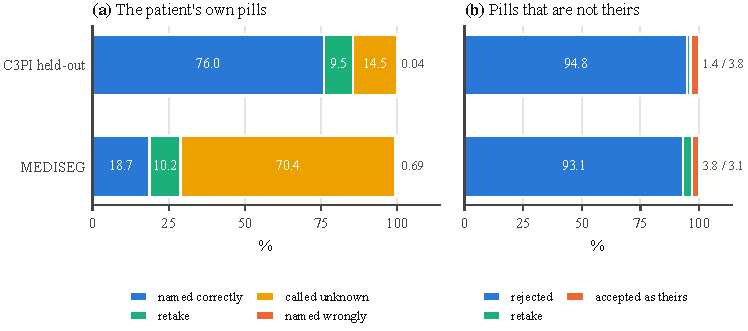
\includegraphics[width=\linewidth]{fig08_open_set_outcomes.pdf}
  \caption{What the patient sees (run 4, embedding only, 10 medicines, 3 enrolment photos). Small shares are listed
    after each bar in legend order. In C3PI conditions most own pills are named correctly and wrong names are rare;
    under acquisition shift the threshold transfers poorly and most own pills are called unknown, which limits useful recognition.}
  \label{fig:openset}
\end{figure}

\subsection{Ablations and hyperparameters}
\label{sec:ablations}

Sequential design changes are summarised in Appendix~\ref{app:calibration}, Table~\ref{tab:ablation}. The combined optimisation changes produce the largest observed improvement. With the new layers at
$10^{-3}$ the embedding collapses to about 3 effective dimensions and validation top-1 stalls at 77\%, while the revised recipe
keeps 12--15 dimensions and reaches 98\% (Figure~\ref{fig:training}). Effective dimensionality is defined as $\exp(-\sum_i q_i\log q_i)$,
where $q_i$ is the fraction of embedding variance along principal direction $i$. It equals 256 for equal variance
and one for a single direction. The decision settings are smooth
(Figure~\ref{fig:calib}): the crop window moves correct names by under one point, and the margin trades correct names
for retakes almost one for one. The imprint weight has a clear optimum (Figure~\ref{fig:identify}b), because a large
$\alpha$ lets false OCR reads promote wrong products. The imprint helps most when the pill's own imprint is actually
read: the correct product ranks first in 92.9\% of those queries, compared with 68.6\% when it is not (Figure~\ref{fig:identify}a).







\begin{figure}[!htbp]
  \centering
  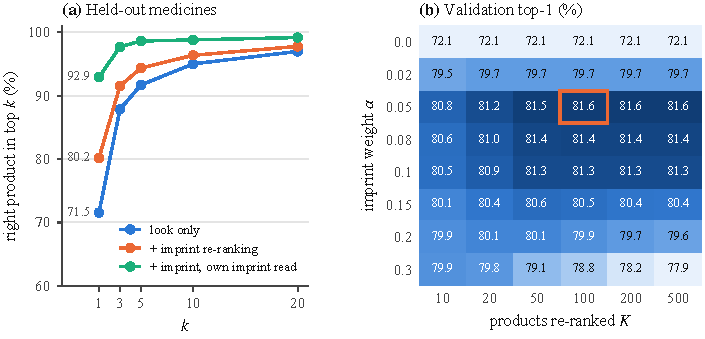
\includegraphics[width=0.92\linewidth,height=0.23\textheight,keepaspectratio]{fig12_identify_topk.pdf}
  \caption{Catalogue identification. (a) Top-$k$ on held-out medicines: the imprint helps most when the pill's own
    imprint is read (92.9\% first vs.\ 68.6\% when it is not). (b) Validation grid for $\alpha$ and $K$; the box marks
    the served setting.}
  \label{fig:identify}
\end{figure}

\FloatBarrier
\subsection{Acquisition transfer and catalogue confidence}
\label{sec:robustness}

Acquisition shift produces the largest loss of useful recognition (Table~\ref{tab:main}, Figure~\ref{fig:openset}). On MEDISEG, top-1 accuracy falls to 48\% and the C3PI-calibrated threshold rejects 70\% of enrolled queries, even though misidentification among enrolled queries remains below 1\%. This decline is associated with image scale: top-1 accuracy is 36--37\% for pills below 100\,px and approximately 62\% above that size (Figure~\ref{fig:robust}a), while additional enrolment photographs provide only partial improvement (Figure~\ref{fig:robust}b).

Catalogue verdicts also differ across sources, with 69.8\% of MEDISEG pills receiving \emph{no confident match} and 7.0\% receiving \emph{possible match}, compared with 75.8\% \emph{possible match} for catalogue pills. The relationship between stated confidence and observed correctness is shown in Figure~\ref{fig:confidence}. Deployment with the smaller CPU reader reduces identification accuracy by one percentage point to 79.2\%, with no increase in the reported rate of wrong naming in the gallery (Table~\ref{tab:main}).

\begin{figure}[!htbp]
  \centering
  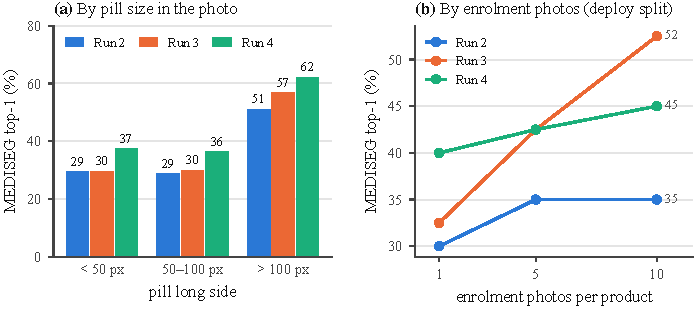
\includegraphics[width=0.92\linewidth,height=0.23\textheight,keepaspectratio]{fig09_robustness.pdf}
  \caption{Robustness on MEDISEG (32 Hong Kong products, other phones, none in training). (a) Top-1 by pill size in the
    photo. (b) MEDISEG's deploy split (40 query pills): more enrolment photos help only partly.}
  \label{fig:robust}
\end{figure}

\begin{figure}[!htbp]
  \centering
  % Match Figure 5's rendered width while preserving this figure's aspect ratio.
  \sbox0{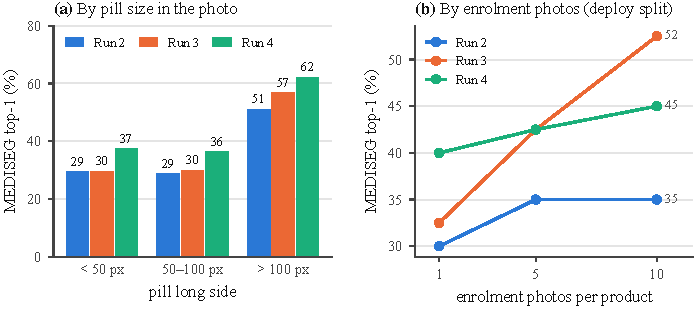
\includegraphics[width=0.92\linewidth,height=0.23\textheight,keepaspectratio]{fig09_robustness.pdf}}
  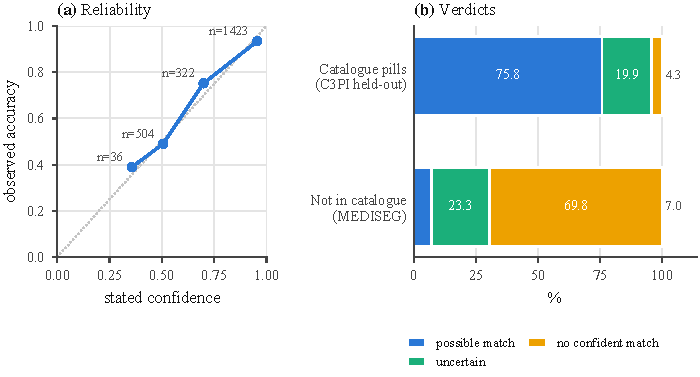
\includegraphics[width=\wd0]{fig13_identify_confidence.pdf}
  \caption{Calibrated confidence for identification. (a) Stated confidence against observed accuracy on held-out
    medicines. (b) Verdicts for catalogue pills and for pills not in the catalogue (MEDISEG).}
  \label{fig:confidence}
\end{figure}

\FloatBarrier
\subsection{Comparison with the ePillID benchmark}
\label{sec:epillid}

The two-sided evaluation averages scores across each front--back pair and includes 626 pairs from 145 types with both sides photographed. The other 47 fold-4 types remain included in the single-photo evaluation; side coverage is shown in Figure~\ref{fig:examples}b.

With one relevant identity per query, MAP corresponds to mean reciprocal rank and MAP@1 to the fraction ranked first. 
In contrast, GAP pools query--candidate scores before calculating average precision, while GAP@1 evaluates top-ranked predictions ordered by score. 
Consequently, a gain in GAP@1 can coexist with lower top-1 accuracy because the measures capture different aspects of ranking and confidence.

Runs 5--7 use the ePillID reference-access setting, permitting references for test types during training while excluding validation groups and types that match their recorded appearance. Retrieval uses the full gallery of 4,902 types (Table~\ref{tab:epillid}).
The embedding alone (MAP 0.57--0.60) falls within the range of the published plain classifiers and remains below the strongest model. 
Re-ranking by imprint, which the paper's model did not use, raises MAP to 0.77--0.78 and GAP@1 to 0.921, above the paper's 0.912, while MAP@1 stays lower (69.0 vs.\ 92.0\%). 
The paper's ablations associate its advantage with its training recipe (contrastive and hard-mined triplet losses with softmax and
ArcFace over side-specific classes, a 2,048-d embedding) alongside its backbone. 
Additional diagnostic comparisons did not recover the gap through crop style, the 64-d pooling step, or local versus global pooling alone.

\begin{table}[!htbp]
  \caption{ePillID benchmark (fold 4, two-sided queries). Runs 5--7 permit test-type references during training but exclude validation groups. The best published model is a ResNet-152 with compact
    bilinear pooling and multi-head metric learning. ``+ imprint'' uses OCR information the published models did not
    use.}
  \label{tab:epillid}
  \centering
  \small
  \begin{tabular}{@{}lccccc@{}}
    \toprule
    & MAP & GAP & MAP@1 & GAP@1 & top-5 \\
    \midrule
    \citet{usuyama2020epillid}, best & \textbf{0.958} & \textbf{0.812} & \textbf{92.0} & 0.912 & -- \\
    \citet{usuyama2020epillid}, plain classifiers & .547--.727 & .241--.448 & 35.7--56.8 & .331--.551 & -- \\
    Ours, run 5 & 0.597 & 0.207 & 45.7 & 0.526 & 77.5 \\
    Ours, run 5 + imprint & 0.780 & 0.598 & 69.0 & \textbf{0.921} & 89.6 \\
    Ours, run 7 + imprint & 0.774 & 0.614 & 67.6 & 0.916 & 89.5 \\
    \bottomrule
  \end{tabular}
\end{table}

\FloatBarrier
\subsection{Error analysis and interpretation}
\label{sec:error-analysis}

\paragraph{Imprint visibility.} A recorded imprint token is recovered on about 47\% of validation photographs, with debossed imprints, small pills and round pills presenting the greatest difficulty. Source visibility labels also identify many unreadable views (Figure~\ref{fig:imprint}), indicating that the available text evidence is constrained by the images themselves.

\paragraph{Look-alike medicines.} When two strengths of one ingredient are enrolled together, one is named as the other in 0.11\% of queries, rising to 0.58\% when shape and colour also match. For pairs sharing an ingredient, the imprint check reduces retakes from 7.5\% to 5.2\% and increases correct naming from 80.1\% to 82.3\%, with a small increase in wrong names. Shared manufacturer prefixes create concentrated errors: tramadol 50\,mg and carvedilol 12.5\,mg are confused in 5.8\% of the corresponding queries despite the imprint check (Figure~\ref{fig:lookalike}). Strength therefore remains associated with the dispensing label rather than confirmed by appearance.

\paragraph{Reader adaptation.} Two LoRA adaptations improve validation imprint recovery from 44.0\% to 53.5\% and from 45.0\% to 50.7\%, respectively. The first produces memorised imprint strings on new pills. The second improves catalogue identification but increases counts of wrong names in the evaluated galleries from 30 to 61. Both adaptations are rejected, as are matching of visually similar characters and separate imprint scoring for each candidate. Full results and representation diagnostics are retained in Appendix~\ref{app:errors}, Table~\ref{tab:negative}.

